%%%%%%%%%%%%%%%%%%%%%%%%%%%%%%%%%%%%%%%%%%%%%%%%%%%%%%%%%%%%%%%%%%%%%%%%%%%%% 
%
% This is a LaTeX file for an A0 poster.
% 
% template poster adapted from https://canizo.org/latex_poster
%
%%%%%%%%%%%%%%%%%%%%%%%%%%%%%%%%%%%%%%%%%%%%%%%%%%%%%%%%%%%%%%%%%%%%%%

%
% Standardised and reproducible analysis of mass spectrometry-based 
% single-cell proteomics data
%
% Poster for the Single Cell Biology conference, November 2020, 
% Hinxton (virtual).
%
% Recent advances in sample preparation, processing and mass
% spectrometry (MS) have enabled the emergence of MS-based
% single-cell proteomics (SCP). However, the lack of computational
% framework limits the optimization and wider application of these
% new technologies. We aim to fill this gap and propose a
% standardised pipeline for the analysis of MS-based SCP data. Our
% packages rely on existing Bioconductor infrastructure, such as
% classes and functions for single-cell RNA sequencing and MS-based
% quantitative proteomics. The first package, `scpdata`,
% disseminates curated SCP data sets for method development and
% benchmarking. The second package, `scp`, implements functions to
% streamline the analysis of SCP data. We demonstrate the
% application of our pipeline by replicating and improving on the
% analyses of two published data sets and show its relevance in the
% processing and interpretation of MS-based SCP data.
%

\documentclass{article}
% To modify the size of the page:
\usepackage[dvips,a3paper,portrait,centering,margin=0.5cm]{geometry}
% To create multiple columns
\usepackage{multicol}

\usepackage[utf8]{inputenc}
% To align images
\usepackage[export]{adjustbox}
% Use captions in minipages
\usepackage{caption}
% Math font
\usepackage{amsmath, amsthm, amsfonts}
% Include figure files.
\usepackage{graphicx}

% Coding fonts
% ------------
% For including R chunks 
\usepackage{listings} 
\lstset{
  language=R,
  basicstyle=\footnotesize\ttfamily\color{vdgray}, % the size of the fonts that are used for the code
  % sensitive=false,
  numbers=left,                   % where to put the line-numbers
  numberstyle=\tiny\color{gray},  % the style that is used for the line-numbers
  stepnumber=1,                   % the step between two line-numbers.
  numbersep=0.1cm,                % how far the line-numbers are from the code
  backgroundcolor=\color{lgray},  % choose the background color. You must add \usepackage{color}
  deletekeywords={stat},
  keywordstyle=\color{blue},      % keyword style
  stringstyle=\color{green},      % string literal style
  xleftmargin=0.5cm,
}
% Create command for highlighting inline code or variables
\newcommand{\hcode}[2][lgray]{{\ttfamily\color{vdgray}\colorbox{#1}{#2}}}

% Colors
% ------
\usepackage{color}
\usepackage[dvipsnames]{xcolor}
% Color panel used throughout the poster
\definecolor{lgray}{rgb}{0.9179688,0.9179688,0.9179688} % #ebebeb
\definecolor{dgray}{rgb}{0.796875,0.796875,0.796875} % #cccccc
\definecolor{vdgray}{rgb}{0.3984375,0.3984375,0.3984375} % #666666
\definecolor{coral}{rgb}{0.9960938,0.4960938,0.3125000} % #ff7f50
\definecolor{blue}{rgb}{0.4218750,0.6484375,0.8007812} % #6ca6cd
\definecolor{green}{rgb}{0.6992188,0.7265625,0.5078125} % #b3ba82
\definecolor{yellow}{rgb}{0.9570312,0.8671875,0.6992188} % #f5deb3

% Bibliography
% ------------
\usepackage{url}
% Adjust space between reference items
\let\OLDthebibliography\thebibliography
\renewcommand\thebibliography[1]{
  \OLDthebibliography{#1}
  \setlength{\parskip}{0pt}
  \setlength{\itemsep}{0pt plus 0.3ex}
}
  
\pagestyle{empty}

\def\to{\rightarrow}


% ===========================================================================

\title{}
\author{}
\date{}

\begin{document}


% ---------------------------------------------------------------------------
% Banner


\begin{center}
\colorbox{lgray}{
  \begin{minipage}{3.7cm}
    \includegraphics[width=1.2\linewidth]{figs/DSC_2812.jpg}
  \end{minipage}
  %&
  \begin{minipage}{.72\textwidth}
    \begin{center}
      % Title 
      \vspace{0.4cm}
      \huge 
      \hspace{1cm}
      \noindent
      \textbf{Standardised and reproducible analysis of mass 
        spectrometry-based single-cell proteomics data} \\
      \vspace{0.4cm}
      % Authors
      \Large \textbf{Christophe Vanderaa, Laurent Gatto} \\
      % Affiliation
      \Large \textit{Computational biology and bioinformatics, de Duve
        Institute, UCLouvain} \\
      % email
      \vspace{0.4cm}
      \normalsize christophe.vanderaa@uclouvain.be \\
      \hspace{1cm}
    \end{center}
  \end{minipage}
  %&
  \begin{minipage}{3.7cm}
      
\includegraphics[width=0.7\linewidth, right]{figs/fnrs.png} \\
      \vspace{0.5cm}
      
\includegraphics[width=1.1\linewidth, right]{figs/ucl.png}
  \end{minipage}
}
\end{center}


% ---------------------------------------------------------------------------
% Summary + conclusion
\noindent
% Summary
\colorbox{yellow}{
  \noindent
  \begin{minipage}[t]{13.7cm}
    \vspace{.15cm}
    \section*{\huge Summary}
    \large 
      Recent advances in sample preparation, processing and mass
      spectrometry (MS) have enabled the emergence of MS-based
      single-cell proteomics (SCP). We have developed a computational
      framework by means of two Bioconductor packages to standardize
      SCP data analysis. It will facilitate the development of 
      dedicated algorithms, for instance to deal with missingness
      and batch effects that are characteristic of this type of data, 
      and will promote the reproducibility of further SCP data 
      analyses.
      
    \vspace{0.1cm}
  \end{minipage}
}
\hspace{0.37cm}
% Conclusion
\noindent
\colorbox{yellow}{
  \begin{minipage}[t]{13.6cm}
    \vspace{.2cm}
    \section*{\huge Take home message}
    \large
      The amount of available MS-based SCP data is rapidly increasing 
      and so is the need for dedicated analysis software. We offer 
      two R/Bioconductor packages. The first package, \hcode[yellow]
      {scpdata}, disseminates curated SCP data sets for method 
      development and benchmarking. The second package, \hcode[yellow]
      {scp}, implements functions to streamline the analysis of SCP 
      data. This work provides the ground for reproducible and 
      rigorous development and benchmarking of new state-of-the-art 
      methods.
    \vspace{0.15cm}
 \end{minipage}
}
\vspace{-1cm}


% ---------------------------------------------------------------------------
% Create a 2 column layout
\setlength{\columnsep}{0.5cm}
\begin{multicols}{2}

% ---------------------------------------------------------------------------
% SCP technology
\noindent
\begin{minipage}[t]{\linewidth}
  \vspace{0.5cm}
  \section*{\huge SCP technology}
  
  SCP is enabled by recent advances in sample preparation, liquid
  chromatography and mass spectrometry. 
  
  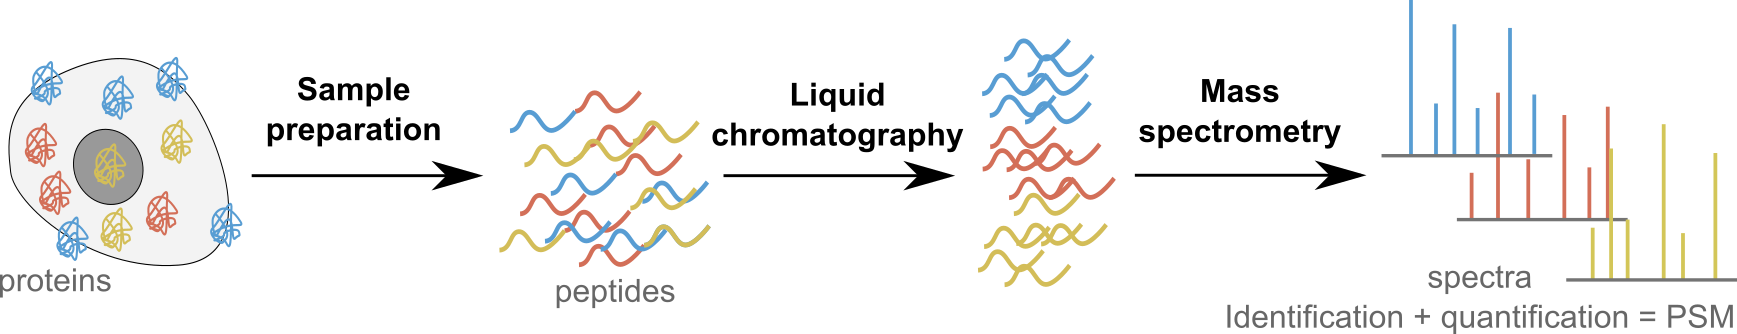
\includegraphics[width=\linewidth]{figs/MS-SCP.png}
  
  \begin{itemize}
  
  \item \textbf{Label-free acquisition}: \textbf{\color{BrickRed}{low 
  throughput}} ($\sim$ 15 samples/day) and \textbf{\color
  {BrickRed}{low identification}} rate, but \textbf{\color{OliveGreen}
  {accurate quantification}} (\textit{e.g.} Zhu et al. 2019 
  \cite{Zhu2019-ja})
  
  \item \textbf{Multiplexed acquisition}: \textbf{\color{OliveGreen}
  {high throughput}} ($\sim$ 200 samples/day), but label 
  \textbf{\color{BrickRed}{cross-contamination}} (\textit{e.g.} SCoPE2
  by Specht et al. 2020 \cite{Specht2020-jm})
  
  \end{itemize}
  
  \textbf{Both methods} generate data with high \textbf{\color{
  BrickRed}{missingness}} and considerable \textbf{\color{BrickRed}
  {batch effects}}.
  
\end{minipage}


% ---------------------------------------------------------------------------
% SCP data framework
\noindent
\begin{minipage}[t]{\linewidth}
  \vspace{0.5cm}
  \section*{\huge SCP data framework}
  
  \large
  SCP data framework = \hcode{SingleCellExperiment}\cite{SCE} +
  \hcode{QFeatures}\cite{QFeatures}
  
  \centering
  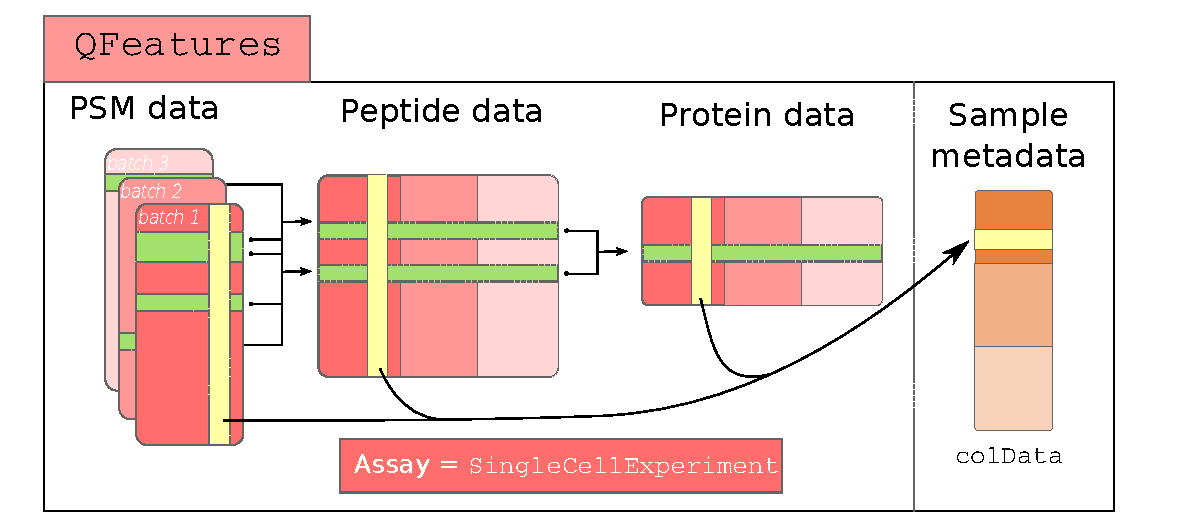
\includegraphics[width=0.7\linewidth]{figs/SCP_framework.pdf}
\end{minipage}

% ---------------------------------------------------------------------------
% scp
\noindent
\begin{minipage}[t]{\linewidth}
  \vspace{0.55cm}
  \section*{\huge \hcode{scp}}
  
  \hcode{scp} implements functions to streamline the analysis of SCP
  data. This code chunk partially reproduces the SCoPE2 analysis by 
  Specht et al. 2020 \cite{Specht2020-jm}.
  
  \begin{lstlisting}
readSCP(quantTable = quantData, metaTable = metaData,
        channelCol = "Channel", batchCol = "Set") %>%
    zeroIsNA(i = 1:4) %>%
    filterFeatures(~ Reverse != "+" & Potential.contaminant != "+") %>%
    subsetByAssay(dims(.)[1, ] > 150) %>%
    computeSCR(i = 1:3, colDataCol = "SampleType",
               carrierPattern = "Carrier",
               samplePattern = "Macrophage|Monocyte") %>%
    filterFeatures(~ !is.na(.meanSCR) & .meanSCR < 0.1) %>%
    aggregateFeaturesOverAssays(i = 1:3, fcol = "peptide",
                                name = paste0("peptides_", names(.)),
                                fun = robustSummary) %>%
    joinAssays(i = 4:6, name = "peptides") %>%
    computeMedianCV(i = "peptides_filter1", proteinCol = "protein",
                    peptideCol = "peptide", batchCol = "Set") %>%
    normalize(i = "peptides", name = "peptides_norm",
              method = "median", na.rm = TRUE) %>%
    logTransform(i = "peptides_norm", name = "peptides_log",
                 base = 2) %>%
    aggregateFeatures(i = "peptides_log", name = "proteins",
                      fcol = "protein", robustSummary) ->
    scp
  \end{lstlisting}

\end{minipage}


% ---------------------------------------------------------------------------
% scpdata
\noindent
\begin{minipage}[t]{\linewidth}
  \vspace{0.55cm}
  \section*{\huge \hcode{scpdata}}
  
  \hcode{scpdata} disseminates curated SCP data sets for method 
  development and benchmarking.
  \vspace{0.1cm}
  
    % latex table generated in R 4.1.0 by xtable 1.8-4 package
    % Wed Oct 21 11:44:14 2020
    \centering
    \scriptsize
    \begin{tabular}{rllllr}
      \hline
     & Title & Description & Species & Date & \# Assays \\ 
      \hline
    1 & specht2019v2 & Specht et al. 2019: macrophage... & Homo sapiens & 2019-12-05 & 179 \\ 
      2 & specht2019v3 & Specht et al. 2019: macrophage... & Homo sapiens & 2019-10-04 & 179 \\ 
      3 & dou2019\_lysates & Dou et al. 2019: HeLa lysates
    ... & Homo sapiens & 2019-10-15 &   3 \\ 
      4 & dou2019\_mouse & Dou et al. 2019: single cells ... & Mus musculus & 2019-10-15 &  13 \\ 
      5 & dou2019\_boosting & Dou et al. 2019: testing boost... & Mus musculus & 2019-10-15 &   7 \\ 
      6 & zhu2018MCP & Zhu et al. 2018 (Mol. Cel. Pro... & Rattus norvegicus & 2018-09-01 &   1 \\ 
      7 & zhu2018NC\_hela & Zhu et al. 2018 (Nat. Comm.): ... & Homo sapiens & 2018-02-28 &   1 \\ 
      8 & zhu2018NC\_lysates & Zhu et al. 2018 (Nat. Comm.): ... & Homo sapiens & 2018-02-28 &   1 \\ 
      9 & zhu2018NC\_islets & Zhu et al. 2018 (Nat. Comm.): ... & Homo sapiens & 2018-02-28 &   1 \\ 
      10 & cong2020AC & Cong et al. 2020 (Ana. Chem.):... & Homo sapiens & 2020-01-02 &   9 \\ 
      11 & zhu2019EL & Zhu et al. 2019 (eLife): chick... & Gallus gallus & 2020-11-04 &  62 \\ 
       \hline
    \end{tabular}
\end{minipage}


% ---------------------------------------------------------------------------
% Batch effects
\noindent
\begin{minipage}[t]{\linewidth}
  \vspace{0.5cm}
  \section*{\huge Batch effects}

  Batch effects are inherent to SCP data since many samples have to 
  be distributed across \textbf{different MS runs}. 
  
  \begin{itemize}
    \item Multiplexed acquisition: 1 run $\sim$ 4-10 cells
    \item Label-free acquisition: 1 batch = 1 cell
  \end{itemize}
  
  Batch effects impact the peptide \textbf{identification} 
  (missingness) and \textbf{quantification}

  \begin{tabular}{p{0.4\linewidth} p{0.4\linewidth}}
    \vspace{0pt} 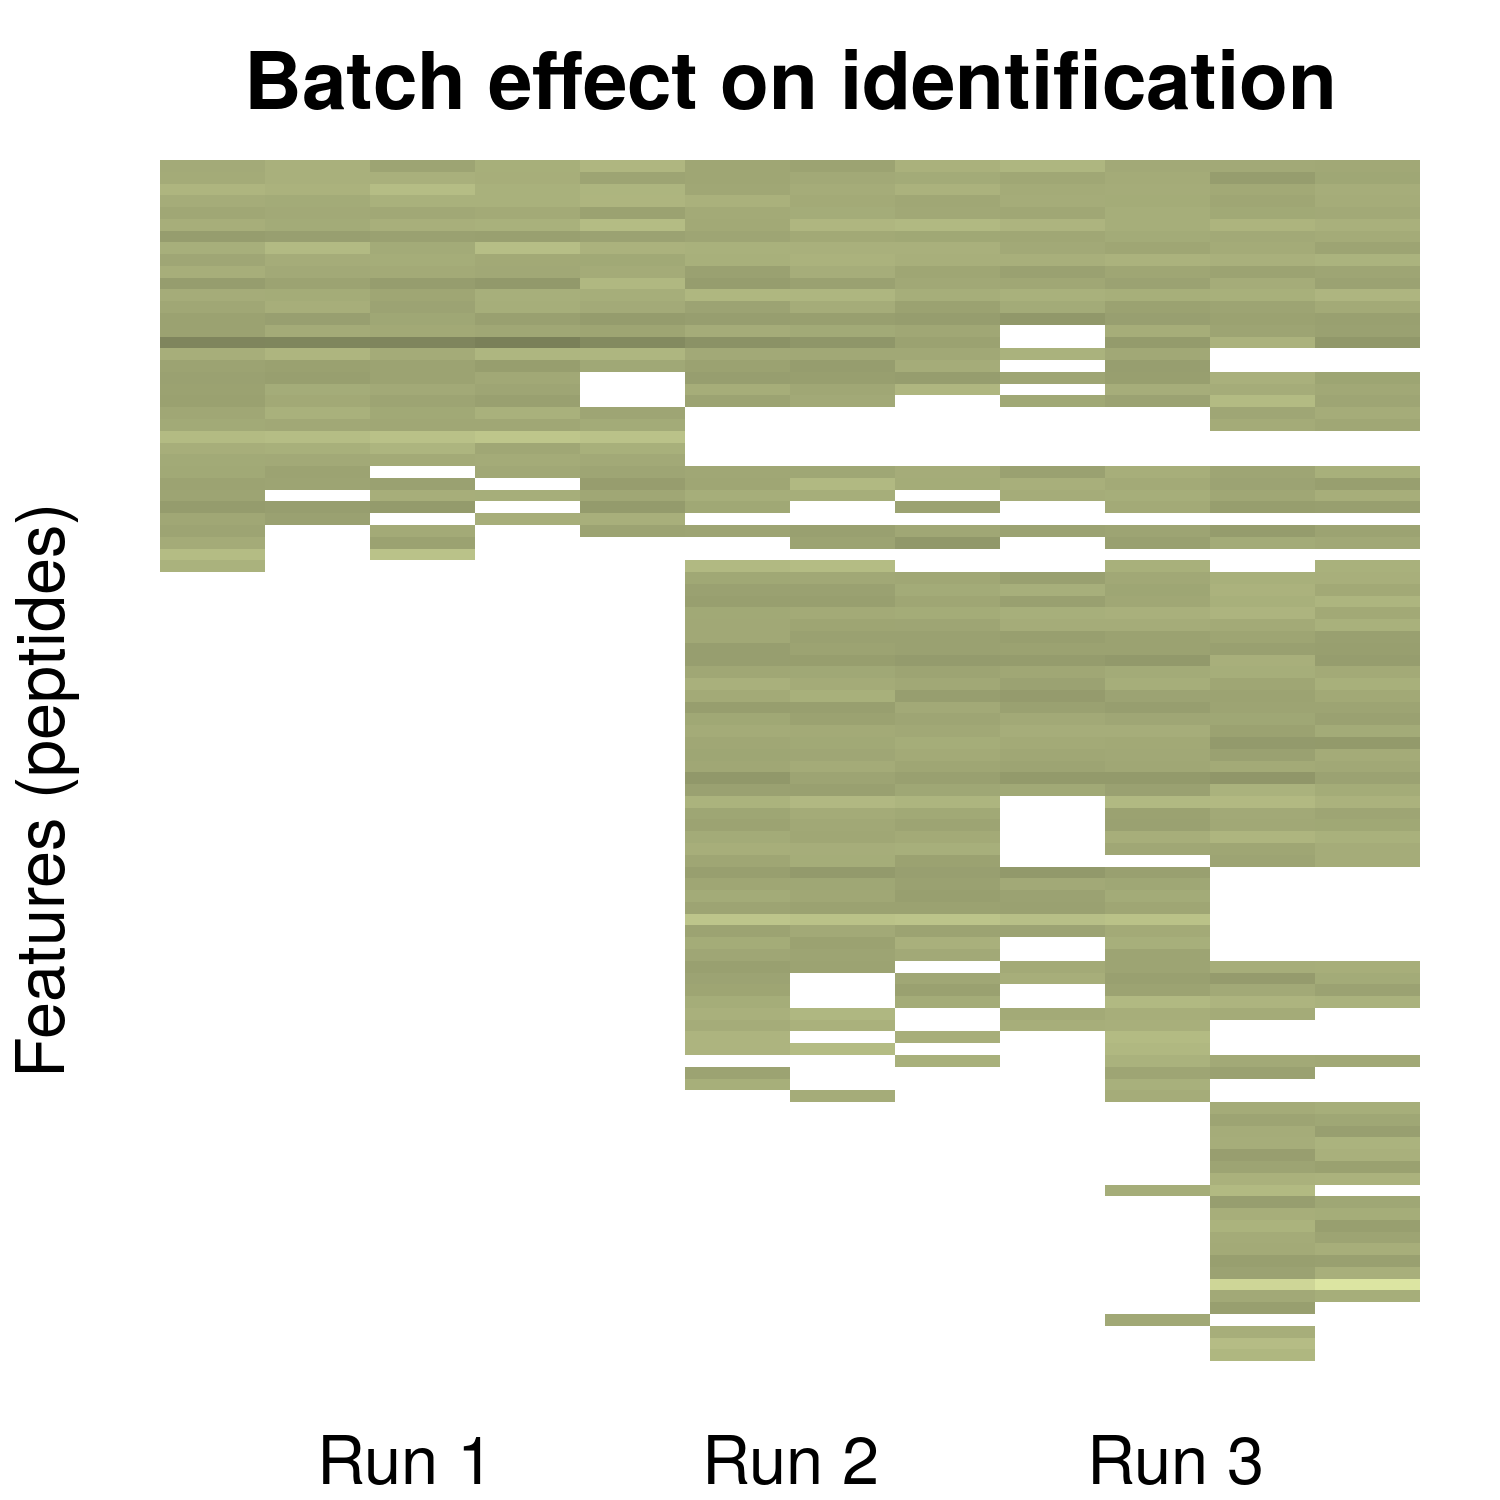
\includegraphics[width=\linewidth]{figs/batch_effects.png} &
    \vspace{0pt} 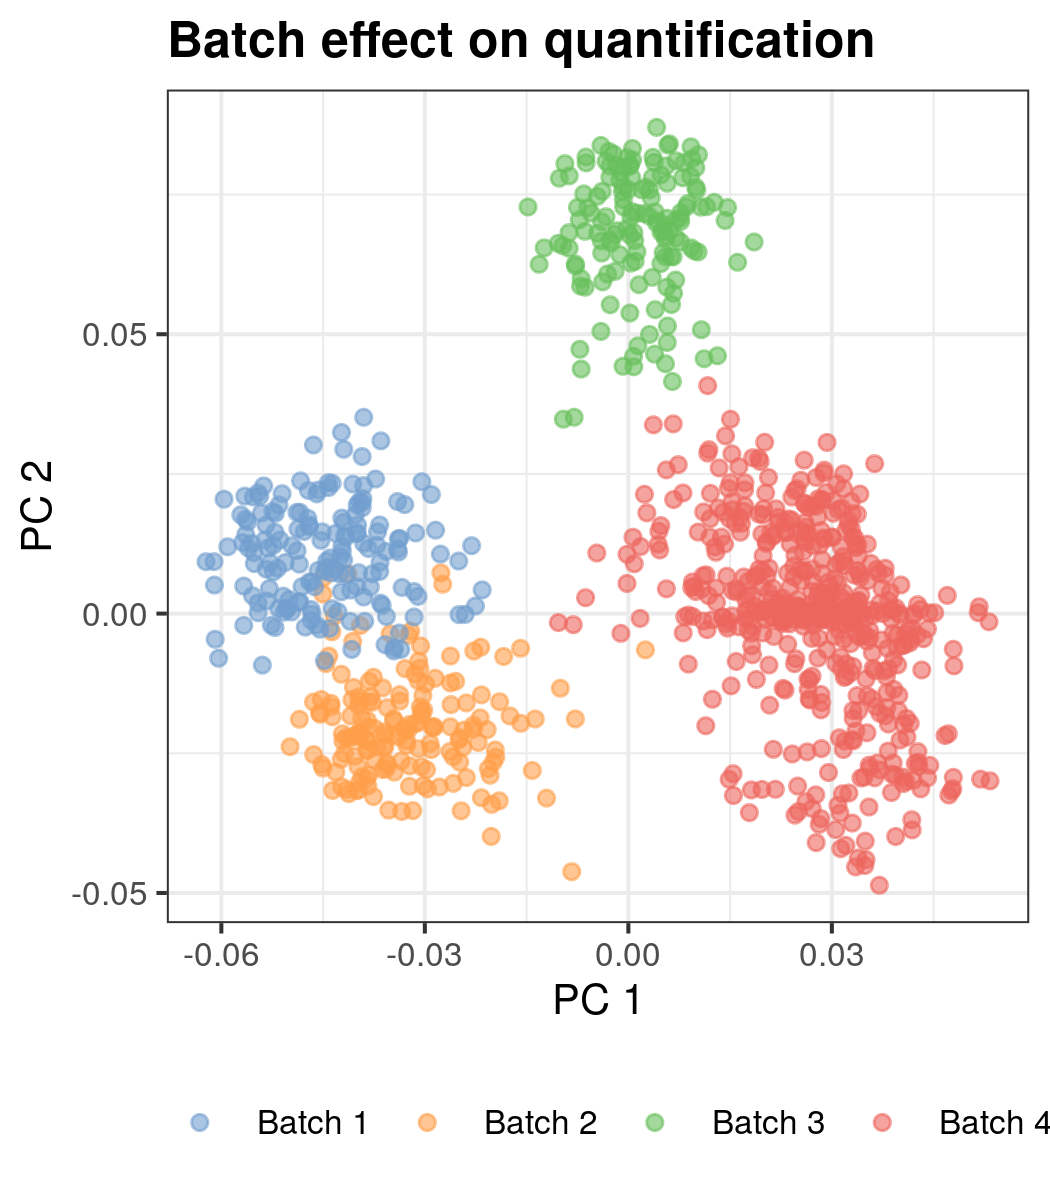
\includegraphics[width=\linewidth]{figs/PCA_batch_effect.png}
  \end{tabular}
  
\end{minipage}


% ---------------------------------------------------------------------------
% Missingness
\noindent
\vspace{-1cm}
\section*{\huge Missingness}
\begin{minipage}[h]{0.35\linewidth}
  
  \begin{itemize}
    \item \textbf{Biological missingness}: some proteins are not 
    expressed in all cells
    \item \textbf{Technical missingness}: low amounts of sample 
    material, instrument sensitivity and batch effects
    \item \textbf{Both}: some proteins are harder to identify (low 
    expression) in one cell type
  \end{itemize}
  
  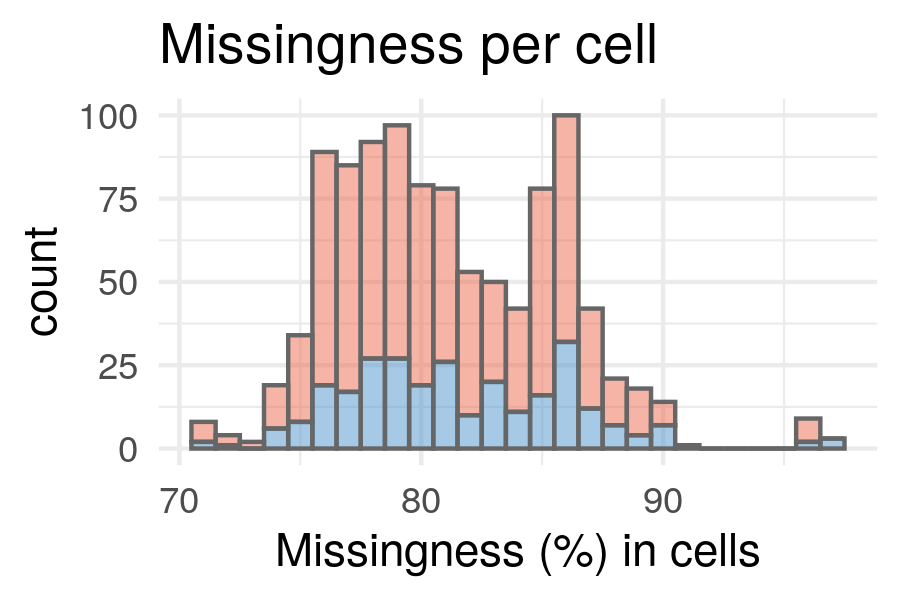
\includegraphics[width=1.2\linewidth]{figs/missing_cell.png}

\end{minipage}\hspace{0.45cm}
\begin{minipage}[h]{0.6\linewidth}
  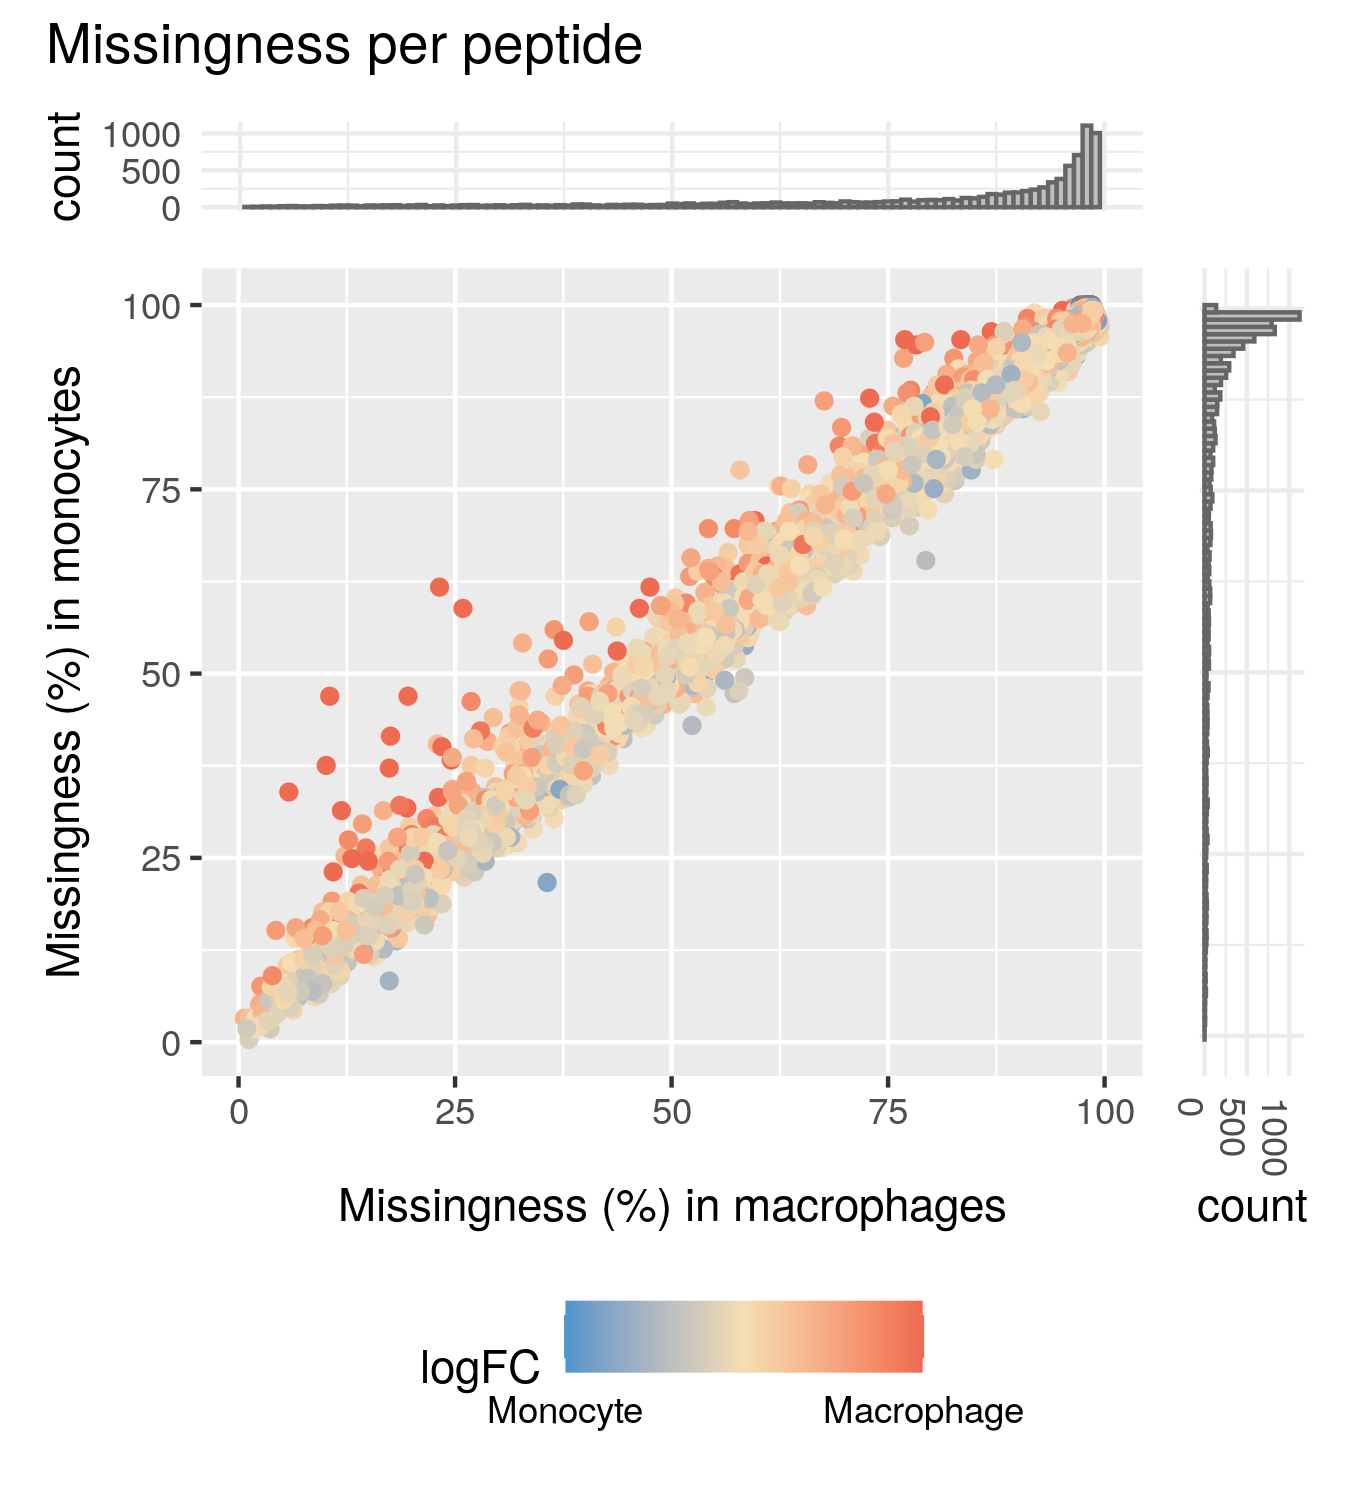
\includegraphics[width=\linewidth]{figs/missing_peptide.png}
  
\end{minipage}


% ---------------------------------------------------------------------------
% Reproducibility 
\noindent
\begin{minipage}[t]{\linewidth}
  \section*{\huge Reproducibility}
  
  \hcode{scp} provides a \textbf{standardized} pipeline for 
  \textbf{unified} and \textbf{reproducible} analysis of SCP data. We 
  used \hcode{scp} to reproduce 2 published analyses:
  
  \begin{itemize}
    \item The analysis by Specht et al. \cite{Specht2020-jm}: 
    \textbf{multiplexed} quantification of 1018 single-cells, either 
    human macropages or monocytes. \textbf{\color{OliveGreen}{Good 
    documentation}} allowed for good replication.
    \item Label-free SCP analysis by Zhu et al. \cite{Zhu2019-ja}: 
    \textbf{label-free} quantification of 28 single-cells from chicken 
    utricles. \textbf{\color{BrickRed}{Poor documentation}} did not 
    allow for replication.
  \end{itemize}
  
\end{minipage}

% ---------------------------------------------------------------------------
% References
\scriptsize
\bibliography{ref.bib} 
\bibliographystyle{ieeetr}

% ---------------------------------------------------------------------------
% Additional notes
\noindent
This work is funded by an Aspirant FRS-FNRS fellowship awarded to 
Christophe Vanderaa.   The poster is available at {\color{blue}
{https://github.com/UCLouvain-CBIO/2020\_11\_09\_posterSCB}}.

% ---------------------------------------------------------------------------
% End of poster
\end{multicols}
\end{document}